\documentclass[11pt]{article}

\usepackage{amsmath}
\usepackage{amssymb}
\usepackage[margin=0.7in]{geometry}
\usepackage{booktabs}
\usepackage{enumitem}
\usepackage{fancyhdr}
\usepackage{graphicx}
\usepackage[table]{xcolor}
\usepackage[hidelinks]{hyperref}
\usepackage{listings}
\usepackage{microtype}
\usepackage{tabularx}
\usepackage{tikz}
\usepackage{titlesec}
\usetikzlibrary{arrows.meta,positioning}
\graphicspath{{docs/lessons/assets/}{../assets/}}

\definecolor{Ink}{gray}{0}
\definecolor{CodeGray}{gray}{0.96}
\hypersetup
{
    pdftitle={ADK Lesson 019: Ultrasonic Range},
    pdfauthor={Kevin Shanahan},
    pdfsubject={Microsecond Echo timing, explicit validity, and physical evidence},
    pdflang={en-US}
}
\pagestyle{fancy}
\fancyhf{}
\lhead{\textsc{ADK Lesson 019}}
\rhead{Ultrasonic Range}
\cfoot{\thepage}
\setlength{\headheight}{14pt}
\setlength{\parindent}{0pt}
\setlength{\parskip}{5pt}
\setlist{nosep,leftmargin=1.45em}
\titleformat{\section}{\Large\bfseries\color{Ink}}{\thesection}{0.5em}{}
\lstdefinestyle{adkcpp}
{
    language=C++,
    backgroundcolor=\color{CodeGray},
    basicstyle=\ttfamily\small,
    keywordstyle=\color{Ink}\bfseries,
    columns=fullflexible,
    keepspaces=true,
    showstringspaces=false,
    frame=single,
    breaklines=true
}
\newcommand{\checkbox}{\(\square\)}
\newcommand{\blank}[1]{\rule{#1}{0.4pt}}
\newcommand{\lessonbox}[1]{%
  \begin{center}
  \fbox{\parbox{0.92\linewidth}{#1}}
  \end{center}}

\begin{document}

\begin{center}
  {\Huge\bfseries Ultrasonic Range}\\[4pt]
  {\Large Time an Echo; publish a qualified reading}\\[8pt]
  \textit{TP-E and three LEDs explain the circuit without Serial.}
\end{center}

\begin{tabularx}{\linewidth}{@{}>{\bfseries}l X >{\bfseries}l X@{}}
Lesson & 019 --- component & Time & 120--180 minutes\\
Prerequisites & Lessons 001--018 & Board & Arduino Mega 2560\\
Evidence & Echo/TP-E and D45--D47 & Status & host verified; bench open\\
Safety & E1: USB-powered low-voltage circuit only\\
\end{tabularx}

\section{Mission}

Build an evidence chain:
\[
\text{Trigger}\rightarrow\text{Echo width}\rightarrow
\texttt{RangeState}\rightarrow\text{visible classification}.
\]
The ranger never turns ``no pulse'' into zero distance. A complete Echo outside
the configured interval is \texttt{OutOfRange}; no accepted Echo is
\texttt{Timeout}; only \texttt{Valid} carries a usable distance.

\lessonbox{\textbf{Boundary.} This sensor is a learning instrument, not a
collision, presence, occupancy, or personnel-safety device. Target shape,
angle, material, air conditions, and module variation affect the result.}

\section{Parts, limits, and wiring}

\begin{tabularx}{\linewidth}{@{}l X@{}}
\toprule
Part & Requirement\\
\midrule
Mega 2560 & USB powered, 5 V logic\\
Ultrasonic module & Exact identified Elegoo EL-SM-001, or bench work blocked\\
Evidence LEDs & Three LEDs, each with its own 220 \(\Omega\) or larger resistor\\
Target & Flat cardboard, initially perpendicular to the sensor\\
Instrument & High-impedance logic probe or oscilloscope\\
\bottomrule
\end{tabularx}

Remove USB power before wiring or moving probe clips. Stop for a hot part,
unstable USB connection, voltage outside the rails, or disagreement between
the module label and this table.

\lessonbox{\textbf{Specimen gate.} The repository has no recorded photograph,
label, lot, or revision for the learner's module. The wiring below is therefore
a conditional circuit for the Elegoo EL-SM-001, whose manufacturer product
page specifies a 5 V DC supply. If the specimen cannot be matched to that
identity and its primary documentation, stop with the bench card open. Do not
infer clone ratings from the HC-SR04-shaped board.}

\begin{tabularx}{\linewidth}{@{}l l X@{}}
\toprule
Signal & Mega & Connection\\
\midrule
Trigger & D40 & module Trigger\\
Echo / TP-E & D41 & module Echo and probe tip\\
Valid evidence & D45 & LED plus resistor to GND\\
Outside evidence & D46 & LED plus resistor to GND\\
Timeout evidence & D47 & LED plus resistor to GND\\
Supply & 5 V, GND & module VCC and GND; probe ground to Mega GND\\
\bottomrule
\end{tabularx}

\begin{center}
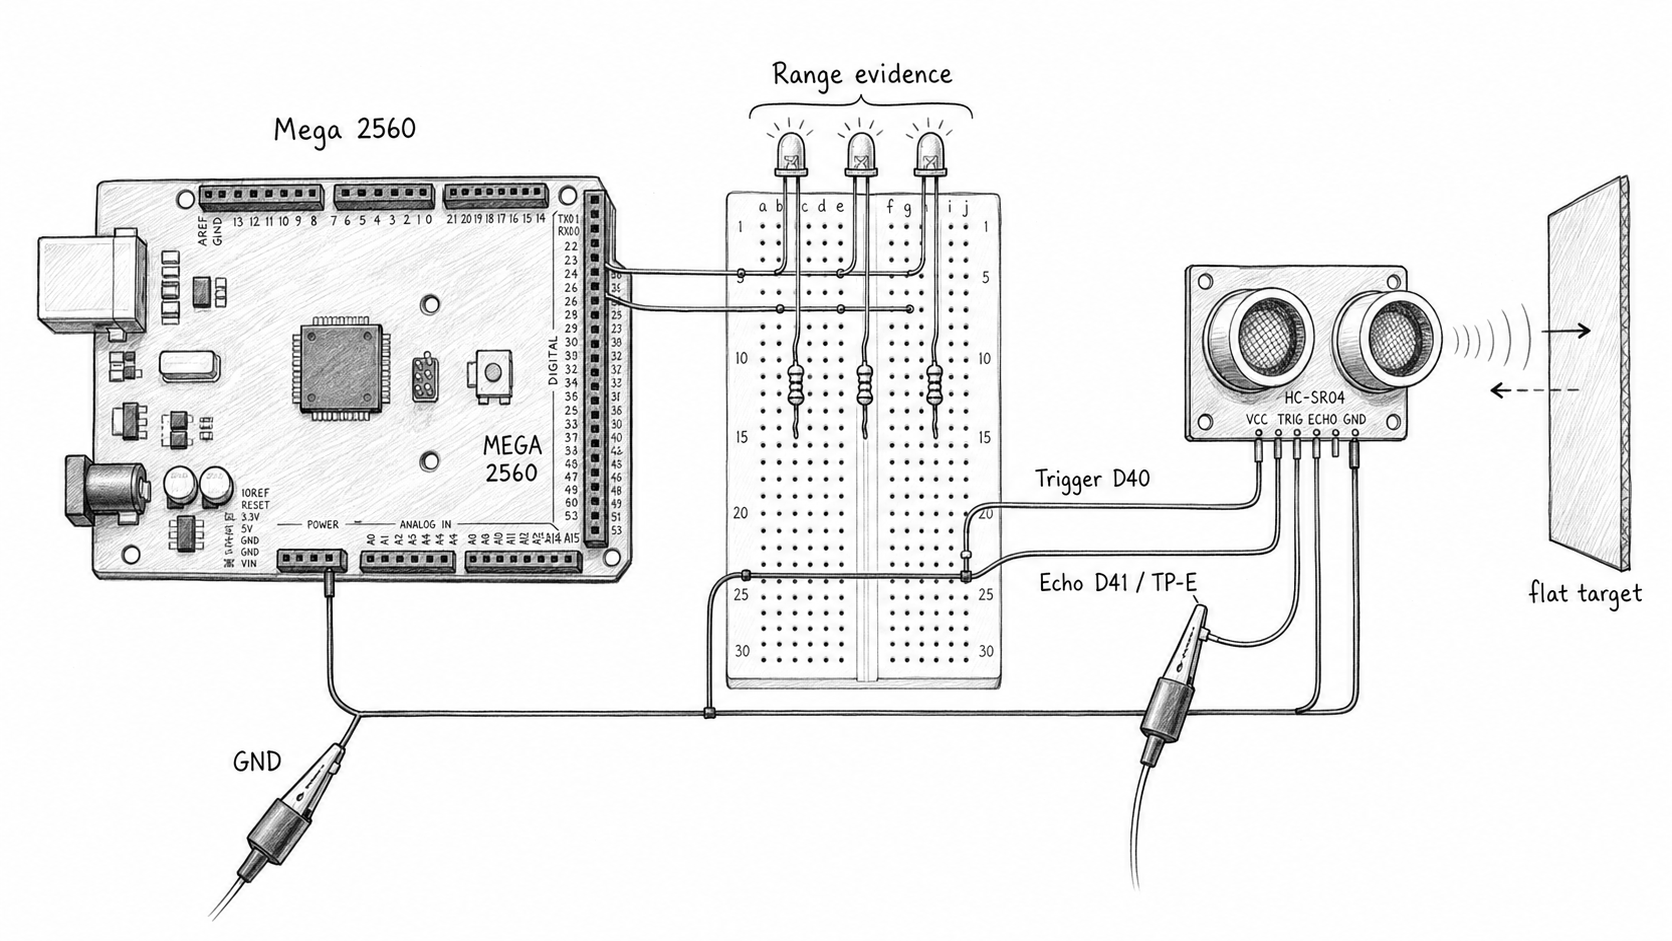
\includegraphics[width=\linewidth]{019-ultrasonic-range-pencil.png}

\small\textit{Alternative text: pencil orientation plate showing a Mega,
breadboard with three resistor-limited LEDs, ultrasonic module, flat target,
Trigger D40, Echo D41/TP-E, and probe ground. The table is authoritative.}
\end{center}

\section{Deterministic model boundary}

\texttt{UltrasonicRanger} is deterministic, non-owning, and hardware
independent. The sketch's endpoints own a \texttt{DigitalOutput} for Trigger
and a \texttt{DigitalInput} for Echo. Every update supplies both time and the
observed Echo level. Resetting the pure model does not release a pin; endpoint
shutdown does.

\begin{tabularx}{\linewidth}{@{}l X@{}}
\toprule
Operation & Contract\\
\midrule
\texttt{initialize()} & return \texttt{Status}; validate the range and timing configuration\\
\texttt{startMeasurement(now, echoHigh)} & return \texttt{Status}; arm from explicit evidence\\
\texttt{update(now, echoHigh)} & return \texttt{Status}; advance from supplied evidence\\
\texttt{reading()} & return stable state, distance, Echo duration, and validity\\
\texttt{reset()} & retain initialization but restore the inert reading state\\
\bottomrule
\end{tabularx}

Check each returned \texttt{Status} with \texttt{ok()}; preserve the complete
status when reporting failure. The configured values are 30 ms Echo timeout,
30 ms maximum Echo duration, 20--4000 mm accepted distance, and
343 \(\mu\)m/\(\mu\)s assumed sound speed. These are software classification
bounds and a model assumption. They do not certify accuracy, prove a specimen
identity, or restate the manufacturer's full operating envelope.

\begin{center}
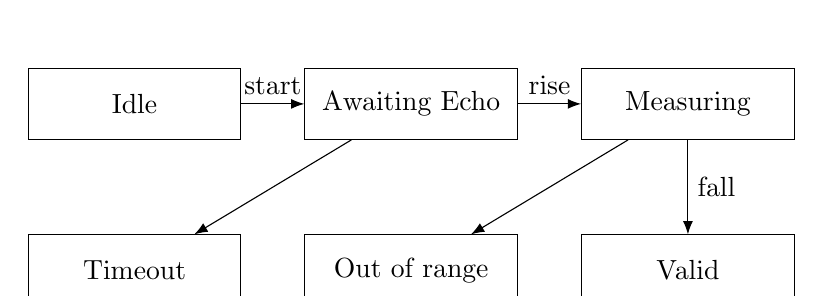
\begin{tikzpicture}[>=Latex,
  state/.style={draw,minimum width=27mm,minimum height=9mm}]
  \node[state] (idle) {Idle};
  \node[state,right=8mm of idle] (rise) {Awaiting Echo};
  \node[state,right=8mm of rise] (high) {Measuring};
  \node[state,below=12mm of high] (valid) {Valid};
  \node[state,left=8mm of valid] (outside) {Out of range};
  \node[state,left=8mm of outside] (timeout) {Timeout};
  \draw[->] (idle)--node[above]{start}(rise);
  \draw[->] (rise)--node[above]{rise}(high);
  \draw[->] (high)--node[right]{fall}(valid);
  \draw[->] (high)--(outside);
  \draw[->] (rise)--(timeout);
\end{tikzpicture}
\end{center}

\section{Narrative run loop}

\begin{lstlisting}[style=adkcpp]
const adk::MicrosecondTimePoint now (micros ());

if (!observeRange (now))
{
    stopSafely ();
    return;
}

const RangeSignal signal = decideRangeSignal ();

if (!showRangeSignal (signal))
{
    stopSafely ();
    return;
}
\end{lstlisting}

Objects appear as runtime, endpoints, evidence LEDs, then ranger. Setup
acquires them in that order. The three LEDs illuminate together for 150 ms as
resource-acquisition evidence. The loop then observes, decides, actuates, and
requests a new reading no sooner than every 60 ms. Idle, valid, timeout, and
out-of-range are all eligible for that next request; a valid distance cannot
stop the measurement cadence and become silently stale.

The 10 \(\mu\)s Trigger pulse uses one explicit bounded delay. Echo timing and
the measurement cadence remain nonblocking. No library behavior allocates,
throws, or reads wall-clock time.

\section{Predict, observe, interpret}

\subsection{Experiment A: acquire separately}

\textbf{Predict.} D45--D47 illuminate together briefly only after their claims
succeed.

\textbf{Observe:} \blank{38mm}.

\textbf{Interpret.} This supports LED and endpoint acquisition; it proves
neither Echo timing nor shutdown state.

\subsection{Experiment B: Trigger and Echo}

Attach probes while unpowered. For a specimen whose primary documentation
calls for it, predict a 10 \(\mu\)s Trigger pulse on D40 and a later high
interval on D41/TP-E. Record:

\begin{tabularx}{\linewidth}{@{}l l l l@{}}
\toprule
Target & Trigger width & Echo width & LED result\\
\midrule
200 mm & \blank{22mm} & \blank{22mm} & \blank{22mm}\\
500 mm & \blank{22mm} & \blank{22mm} & \blank{22mm}\\
1000 mm & \blank{22mm} & \blank{22mm} & \blank{22mm}\\
\bottomrule
\end{tabularx}

Estimate distance using
\[
d_{\mathrm{mm}}\approx
\frac{t_{\mathrm{echo},\mu s}\times343}{2000}.
\]
Division by two accounts for the outward and return path. Compare the estimate
with the LED category and ruler distance. Do not call this calibration.

\subsection{Experiment C: distinct invalid results}

Turn the flat target away without touching the powered circuit. A missing
accepted Echo should select D47. Move a complete target deliberately outside
the documented interval only if the bench permits it; that should select D46.
Record what was observed, not what software was expected to do.

\subsection{Experiment D: safe state}

Invoke the shutdown exercise. D40 must be low before it becomes input/high
impedance; TP-E is no longer sampled; all evidence LEDs are inactive. Check
Trigger electrically. An LED being off does not prove Trigger safe state or
claim release.

\section{Diagnosis}

\begin{tabularx}{\linewidth}{@{}l X@{}}
\toprule
Observation & Check next\\
\midrule
No startup light walk & endpoint conflict, polarity, resistor, and initialization status\\
Trigger present; Echo absent & module supply, common ground, target angle, and exact module\\
Echo present; fault LED & pulse width, timeout boundary, and probe reference\\
Valid LED; implausible distance & target geometry, Echo width, sound-speed assumption, units\\
Outside LED at ordinary range & configured limits and integer conversion\\
Trigger remains driven after stop & safe-state failure; remove USB and record the deviation\\
\bottomrule
\end{tabularx}

\section{CLI and bench record}

\begin{verbatim}
make host-test
make arduino-Lesson019UltrasonicRange
make firmware-size EXAMPLE=Lesson019UltrasonicRange
make upload EXAMPLE=Lesson019UltrasonicRange PORT=/dev/ttyACM0
make lessons
make lessons-check
make site-check
\end{verbatim}

\textbf{Use with.} The
\href{https://spincyc.github.io/adk/lessons/019.html}{HTML reference} carries
searchable API notes, corrections, and direct downloads. This PDF is the
printable experiment, prediction worksheet, diagnosis table, and acceptance
record. Shared safety limits, pins, prerequisites, and API facts appear in
both.

\begin{itemize}
  \item
    \href{https://github.com/spincyc/adk/blob/main/src/ultrasonic_ranger.h}
         {UltrasonicRanger public header} and
    \href{https://github.com/spincyc/adk/blob/main/src/ultrasonic_ranger.cpp}
         {implementation}
  \item
    \href{https://github.com/spincyc/adk/blob/main/src/pulse_input.h}
         {PulseInput public header} and
    \href{https://github.com/spincyc/adk/blob/main/src/pulse_input.cpp}
         {implementation}
  \item
    \href{https://github.com/spincyc/adk/blob/main/tests/test_ultrasonic_ranger.cpp}
         {deterministic host tests} and
    \href{https://github.com/spincyc/adk/blob/main/examples/Lesson019UltrasonicRange/Lesson019UltrasonicRange.ino}
         {canonical Mega 2560 example}
\end{itemize}

\textbf{Software:} commit \blank{34mm}; Arduino CLI \blank{26mm};
AVR core \blank{26mm}; flash \blank{20mm}; RAM \blank{20mm}.

\textbf{Bench acceptance---open until measured}

\begin{itemize}
  \item \checkbox\ Exact Mega and ultrasonic module recorded.
  \item \checkbox\ Unpowered wiring and each LED resistor checked.
  \item \checkbox\ 5 V rail and module supply measured.
  \item \checkbox\ D40 Trigger width measured.
  \item \checkbox\ D41/TP-E widths recorded for three ruler distances.
  \item \checkbox\ Valid, out-of-range, and no-Echo evidence distinguished.
  \item \checkbox\ Reset, shutdown, resource reuse, and USB removal observed.
  \item \checkbox\ Trigger safe state checked separately from LEDs.
\end{itemize}

Supply \blank{20mm}; instrument \blank{34mm}; target \blank{28mm};
date \blank{22mm}; reviewer \blank{30mm}. Deviations: \blank{65mm}.

\lessonbox{\textbf{Current result: host verified; hardware acceptance open.}
Deterministic tests, compilation, and blank worksheets are not physical
verification.}

\section{Primary references}

\begin{itemize}
  \item
    \href{https://www.elegoo.com/en-gb/products/elegoo-5pcs-hc-sr04-ultrasonic-module-distance-sensor-compatible-with-arduino-uno-mega-r3-nano-robot-xbee-zigbee}
         {Elegoo EL-SM-001 product specification}: conditional source for the
         named module's 5 V supply, stated range, acoustic frequency, and model
         identity.
  \item
    \href{https://www.elegoo.com/blogs/arduino-projects/elegoo-hc-sr04-ultrasonic-sensor-module-tutorial}
         {Elegoo HC-SR04 documentation index}: manufacturer-hosted datasheet
         route; match it to the physical specimen before bench work.
  \item
    \href{https://docs.arduino.cc/resources/datasheets/A000067-datasheet.pdf}
         {Arduino Mega 2560 Rev3 datasheet}: official board power and D40--D47
         connector identities.
\end{itemize}

\section{Extend the evidence}

\begin{enumerate}
  \item Record how angled cardboard changes Echo validity without changing code.
  \item Replay the same timestamp and level trace twice and compare readings.
  \item Explain why clamping an invalid distance would erase useful evidence.
  \item Design a fourth diagnostic that adds information not already present at
        TP-E or the three result LEDs.
\end{enumerate}

\end{document}
